\documentclass[a4paper]{article}
\usepackage{mystyle}

\begin{document}

\customtitle{Fluctuation Strength Sample Size Determination}

\section{Introduction} % (fold)
\label{sec:introduction}

This documents describes the sample size calculations regarding the fluctuation
strength experiments when the effect of the modulation frequency change is
assessed.

% section introduction (end)

\section{Considerations} % (fold)
\label{sec:considerations}

Several parameters are needed to calculate the sample size. The standard
deviation can be obtained from Figure~\ref{fig:fsvsmf}, where the interquartile
ranges for all the fluctuation strength responses to the three types of stimuli
are presented. The maximum interquartile range, which corresponds to the 8 Hz FM
tone, is about 1.6 vacil. Using this value as the whole range for the values
(i.e., approximately 6 standard deviations), it can be derived that the standard
deviation is of about 0.26 vacil. The median value for this point is of about
0.4 vacil. Furthermore, the minimum distance between values for Figure
\ref{fig:fsvsmf}c is of about 0.15 vacil; this value will be used to calculate
the confidence interval precision.

\begin{figure}[ht]
    \centering
    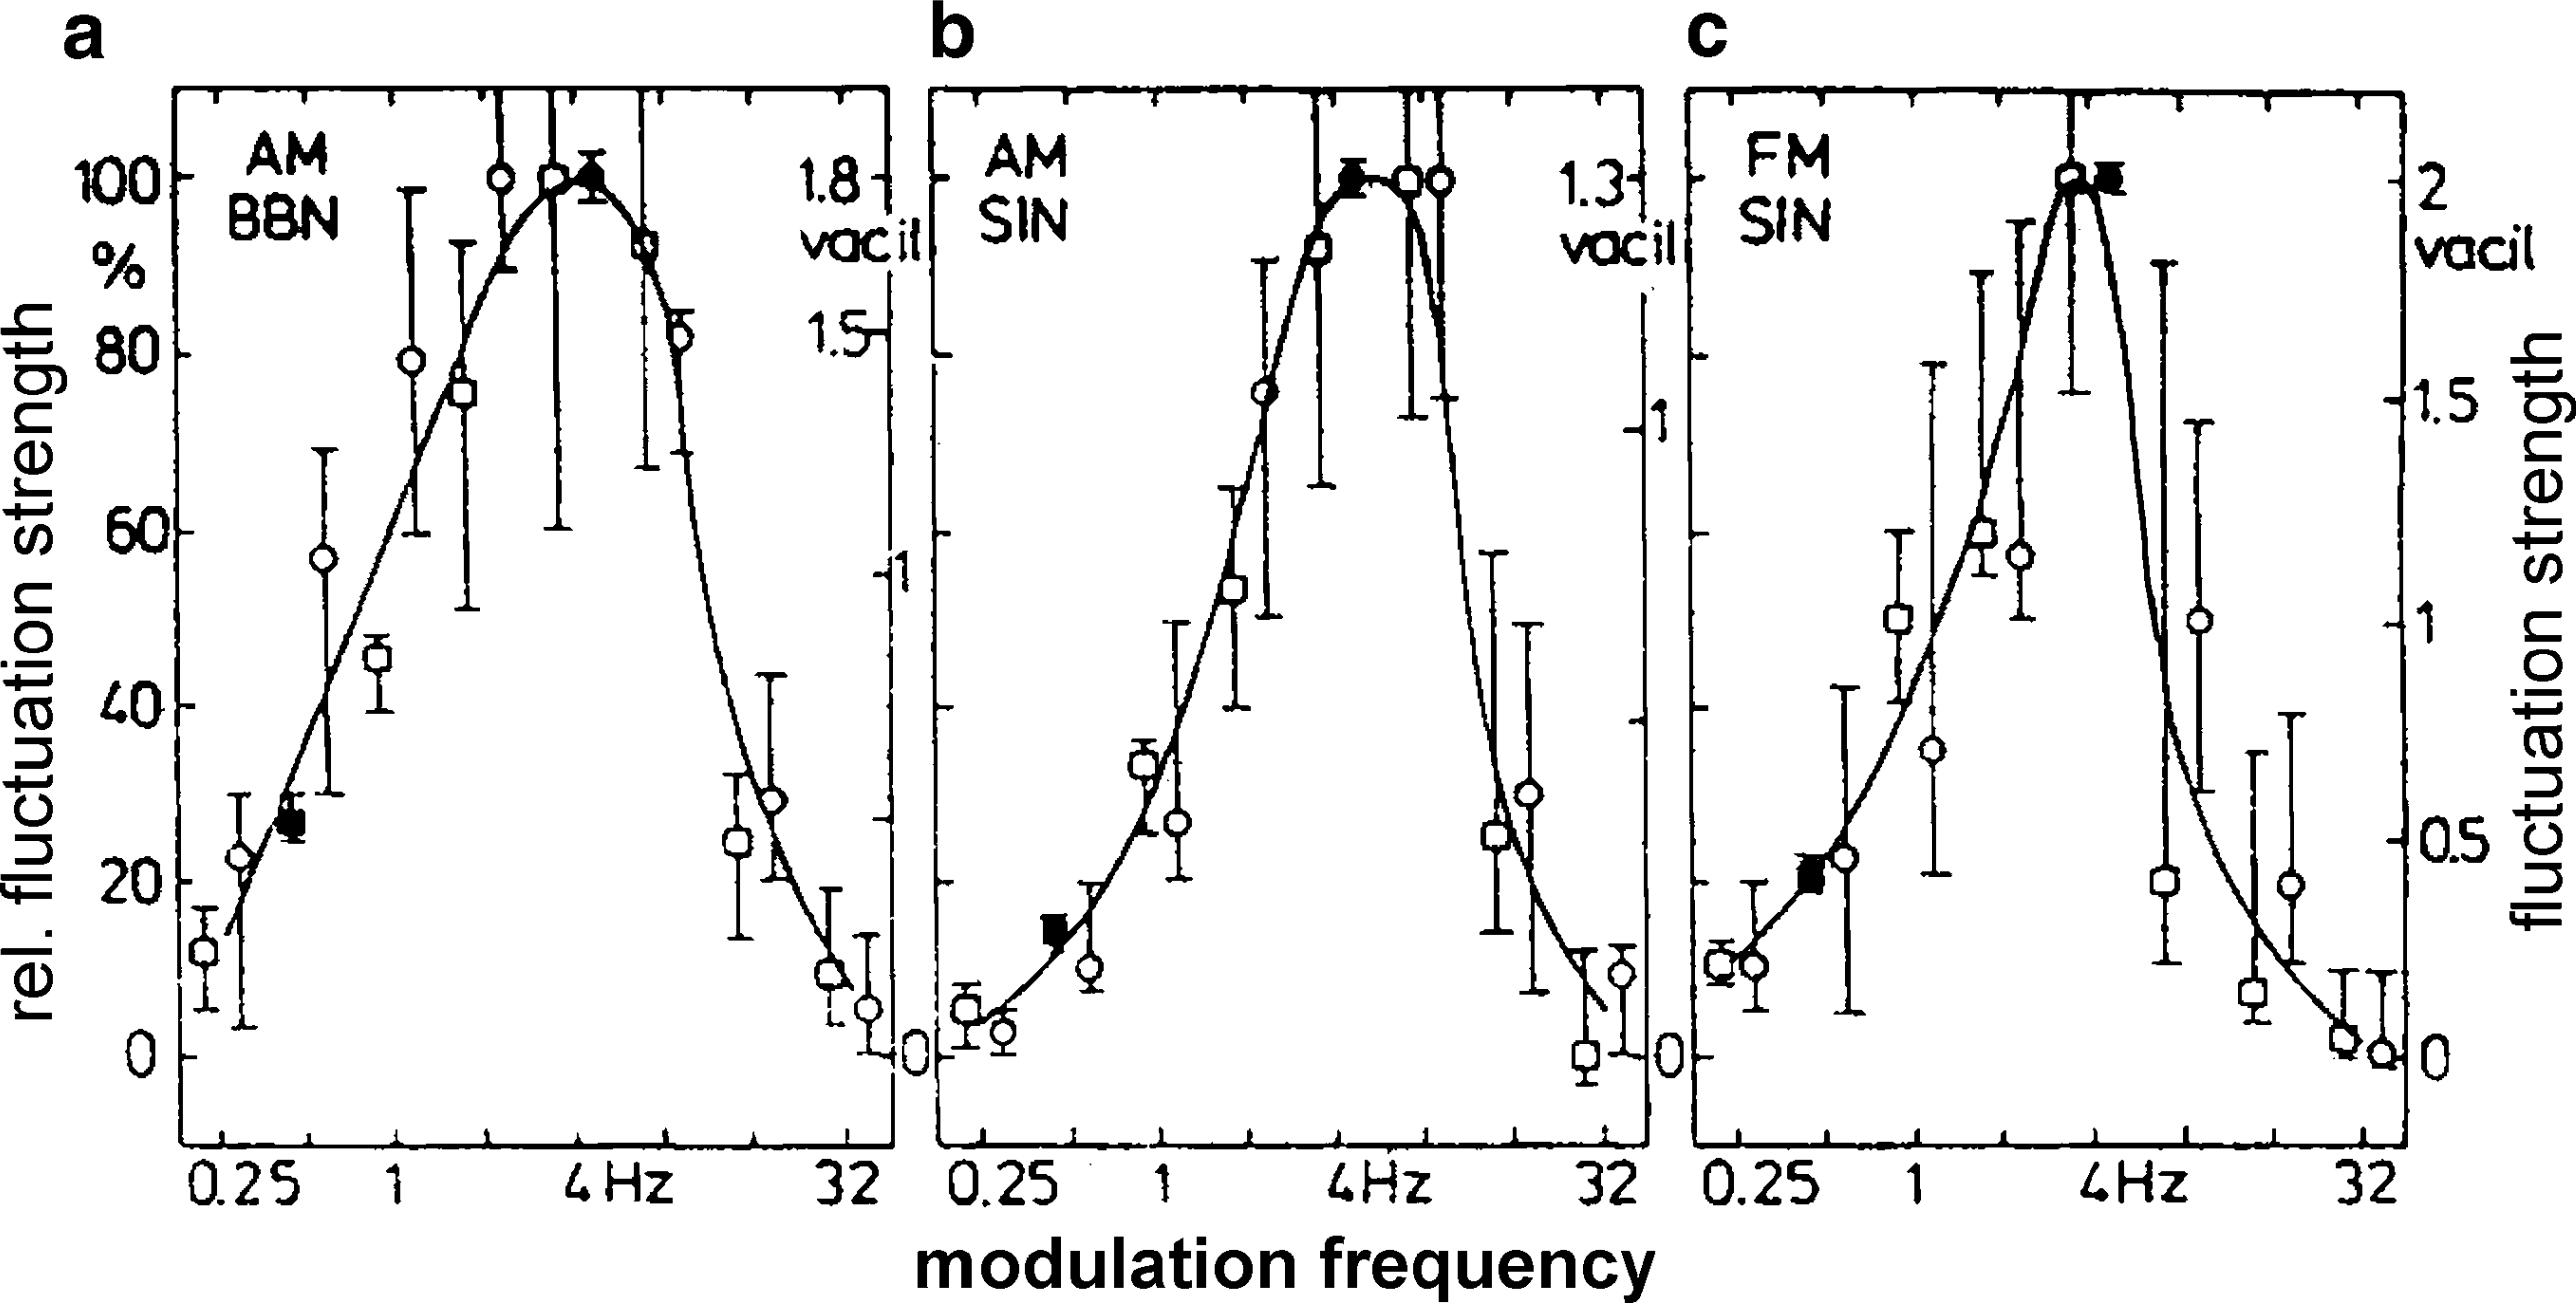
\includegraphics[height=8cm]
        {Mueller2012Handbook/img/FluctuationStrengthVsModulationFrequency}
    \caption{Fluctuation strength of three modulated sounds as a function of
        modulation frequency. (a) Amplitude-modulated broad-band noise of 60-dB
        SPL and 40-dB modulation depth; (b) amplitude-modulated 1-kHz tone of
        70-dB SPL and 40-dB modulation depth; (c) frequency-modulated pure tone
        of 70-dB SPL, 1500-Hz center frequency and $\pm$ 700-Hz frequency
        deviation;~\cite[pp. 248]{Fastl2007Psychoacoustics}}
\label{fig:fsvsmf}
\end{figure}

% section considerations (end)

\section{Calculations} % (fold)
\label{sec:calculations}

\subsection{Confidence Interval} % (fold)
\label{sub:confidence_interval}

Using Equation~\ref{eq:ci} a sample size can be calculated. Using
$z_{\alpha/2} = 2$ (95\% confidence interval), $\sigma = 0.26$  and E = 0.15,
a value of 12 is obtained.

\begin{equation}
  n = \Big( \frac{z_{\alpha/2} \cdot \sigma}{E} \Big) ^2
\label{eq:ci}
\end{equation}

% section calculations (end)

\custombibliography{}

\end{document}
